\subsection{Implementation and dependencies}
\bioptim is the top layer of a succession of dependencies (\biorbd: dynamics and MSK modeling; \casadi: automatic differentiation; \ipopt/\acados: optimization; \bioviz: visualization).
Within this software suite, \bioptim 's main role is to shape the problem to allow its dependencies to communicate efficiently, while providing an intuitive and flexible interface to the user (Fig.~\ref{fig:dependencies}).
Therefore, it was written in Python for its flexibility and its widespread use among researchers.
However, all intensive calculations behind the interface are performed in \comment{C/C++}{Bien que ça ne soit pas faut, je trouve ça légèrement misleading... les calculs sont en réalité fait dans un graph casadi (qui est effectivement en C), mais la partie C/C++ rapide, c'est donc surtout en Eigen qu'on la ressens}, keeping \bioptim both fast and easy to customize.

\begin{figure}[t!]
\centering
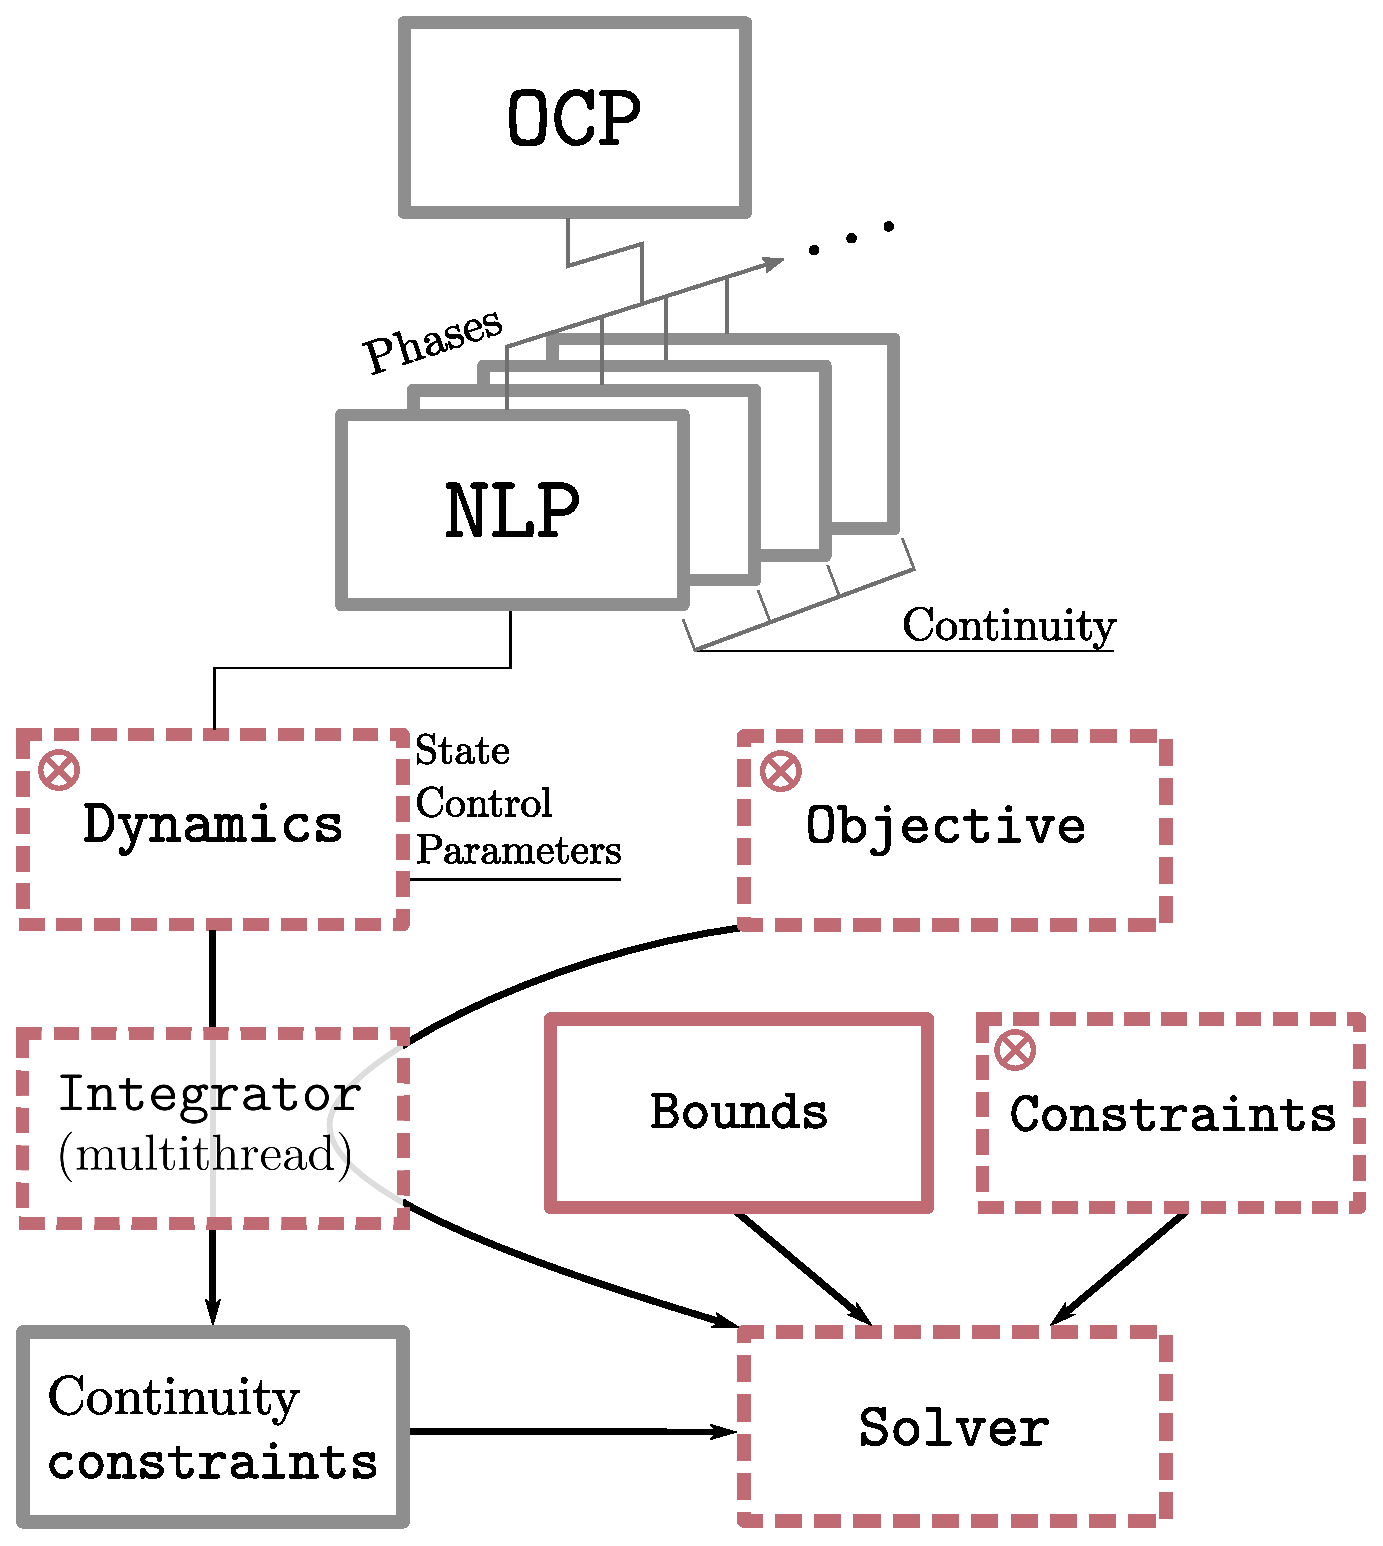
\includegraphics[width=0.9\columnwidth]{figures/design.eps}
\caption{\bioptim design flowchart.}
\label{fig:dependencies}
\vspace*{-0.5cm}
\end{figure}


\subsection{Design}
\bioptim shapes and solves optimal control problems whose two required entries are a model (.\textit{bioMod} file) and an OCP.
The model file contains the geometrical characteristics, the segment inertias, the markers, the actuators of the model (muscles and joint torques possibly with angle/angular velocity/torque relationships) as well as bounds on joint kinematics and torques. 
It also allows the user to design or import meshes for visualization purposes.
The OCP is implemented as a combination of nonlinear problems (NLPs) for allowing the formulation of multi-staged OCPs. 
Each NLP has the following attributes: a dynamics type, an \comment{objective function}{set? car ce n'est pas obligatoire, même chose pour constraints}, constraints, a number of shooting points, the duration of the problem and \comment{initial guesses}{et les bounds? ça peut entrer dans constraints, mais c'est quand même légèrement différent...}.
Based on these inputs, \bioptim properly sets up the multiple shooting transcription of the OCP, with appropriate continuity constraints in the case of multiple NLPs, and shapes it up to feed the chosen non-linear solver (\ipopt or \acados). 

\subsubsection{Dynamics types}
The dynamics type defines which variables are states ($\state$), which ones are controls ($\control$) and which ones are \comment{parameters}{À ignorer si c'est fait plus tard: serait-il pertinent de mentionner que la différence fondamentale entre controls et parameters c'est que un est temps indépendant?} ($\param$).
Then, it implements the ordinary differential equation governing the state transition:

\[
\dstate = f(\state, \control, \param).
\addtag
\label{eq:state_transition}
\]

\noindent More than 10 dynamics are implemented in \bioptim \footnote{\href{https://github.com/pyomeca/bioptim/blob/master/bioptim/dynamics/dynamics_functions.py}{github link}}, among which the controls can be muscle excitations, muscle activations or joint torques, the states can be muscle activations and/or joint kinematics.
They can include contact points, external forces, etc.
Even if these dynamics types exhaustively span the current usages in biomechanics, a custom dynamics type is also pre-implemented to easily customize problems.

\subsubsection{Objective functions}
In line with the optimal control formalism, there are two main types of objective functions, namely Lagrange and Mayer. 
Lagrange types are running objectives, integrated over the NLP duration. Mayer types are time-specific objectives. 
Classically, they correspond to a terminal objective, but to be more versatile, they can be defined at any instant in \bioptim\comment{.}{Spécifier que ce n'est pas le cas avec ACADOS?}

These objective functions can depend on any of the optimization variable, \textit{i.e.} the controls, the states, the parameters and the duration of the problem. 
A lot of objective function types are already implemented in \bioptim ($>\!20$), among which tracking\:/\:minimizing, on states\:/\:controls\:/\:markers\:/\:contact\:forces\:/\:problem\:duration, etc. 
Should one go missing, a custom objective type is also possible to define.

When declaring the desired list of objective functions for a given NLP, each objective function type is associated with a weight, and the user can choose on which components of the vector variables the objective must apply. 
If applicable (for tracking objective functions mainly), the user must also specify the numerical target of the objective.

\subsubsection{Constraints}
Classically, constraints are hard penalties of the optimization problem, i.e., a solution will not be considered optimal, unless every constraint (equality or inequality) is met.
In \bioptim, there exist two classes of constraints: the \texttt{Bounds} and the \texttt{Constraint}.
Essentially, the \texttt{Bounds} are constraints directly related to the states and the controls.
They are useful for defining model-related constraints such as kinematic, torque or muscle excitation\:/\:activation limits. 
The \texttt{Constraint} class contains a variety of already implemented constraints.
Among them, the user will find the constraint equivalents of every objective function in addition to  other ones, commonly useful in biomechanical problems (e.g. non-slipping contact point, non-linear bounds on torque depending on the state, etc.).
Should one go missing, a custom constraint type is also possible to define.